%%%%Draft version
% \documentclass[12pt,letterpaper,spanish,draft,twoside]{book}
%%%%Final version
\documentclass[12pt,letterpaper,spanish,twoside,final]{book}

\usepackage{Thesis}
% New bibliography system: biber (No bibtex needed)
\usepackage[
  backend=biber
]{biblatex}
\addbibresource{bibliografia.bib}

%%%%For producing modified TOC with less space inbetween.
\usepackage{tocloft}
\setlength\cftparskip{-2pt}
\setlength\cftbeforesecskip{1pt}
\setlength\cftaftertoctitleskip{2pt}

%\includeonly{dedicatoria} %Por debug solo compila un capitulo

\begin{document}

\selectlanguage{spanish}

%%%%Change numbering to roman
\clearpage \pagenumbering{roman}
%\listoftodos

\begin{titlepage}
\vspace*{-1.5cm}
\noindent\makebox[\textwidth]{%
\begin{tabular}{cc}
\multirow{6}{*}{
\includegraphics[scale=.12]{img/escudoUNAM}} \\
\\\\
 & \uuline{\textsc{\large Universidad Nacional Autónoma de México}}\\[.5cm]
 & \textsc{Facultad de Estudios Superiores Acatlán}\\
\\
\\
\end{tabular}}

\vspace{1.5cm}
\noindent\makebox[\textwidth]{%
\begin{tabular}{c@{\hspace{1.5cm}}||@{\hspace{1cm}}lr}
 & \multicolumn{2}{c}{\textsc{\large ``Modelado Gráfico de un Cuerpo}}\\
 & \multicolumn{2}{c}{\textsc{\large Neumático con OpenGL a Base de}}\\
 & \multicolumn{2}{c}{\textsc{\large Ecuaciones Diferenciales''}}\\[1cm]
 & \multicolumn{2}{c}{\textsc{\Large{T \ E  \ S \ I \ S}}}\\[1cm]
 & \multicolumn{2}{c}{\textsc{\large que para obtener el grado de:}}\\[1cm]
 & \multicolumn{2}{c}{\textsc{\large Licenciado en Matemáticas}}\\
 & \multicolumn{2}{c}{\textsc{\large Aplicadas y Computación}}\\[1cm]
 & \multicolumn{2}{c}{\textsc{\Large{P \ R \ E \ S \ E \ N \ T \ A}}}\\[1cm]
 & \multicolumn{2}{c}{\textsc{\Large Jorge Antonio García Galicia}}\\[2cm]
 & \textsc{Director de Tesis:}\\
 & & \textsc{Dr. María del Carmen Villar Patiño\ \ \ \ \ \ \ \ \ \ \ }\\[1.5cm]
 & México, D.F. & 2008
\end{tabular}
}
\end{titlepage}

% \newpage
% \thispagestyle{empty}
% \mbox{}

\cleardoublepage

\thispagestyle{empty}
\vspace*{8cm}
\begin{flushright}
\textit{A toda la gente que paga sus impuestos\\
y que cumple con su trabajo en paz.}
\end{flushright}                 

% \newpage
% \thispagestyle{empty}
% \mbox{}

\cleardoublepage

\chapter*{Agradecimientos}

{\small
Agradezco al Consejo Nacional de Ciencia y Tecnología (\textsc{conac}y\textsc{t}), por apoyar esta investigación con la beca \textsc{cvu}--XXXX para estudios de Maestría en la Universidad Nacional Autónoma de México.

Agradezco también al Departamento de Ciencias de la Computación del Instituto de Investigaciones en Matemáticas Aplicadas y en Sistemas por permitirme hacer uso de sus instalaciones y por todos los recursos materiales con los que me apoyaron.

Y por supuesto, gracias\ldots

A toda la gente que paga sus impuestos y que cumple con su trabajo en paz.
}

\cleardoublepage

\chapter*{Resumen}
Este trabajo trata de como visualizar campos escalares que han pasado por un proceso de digitalización. En particular se usa una técnica de graficación por computadora conocida como visualización por superficies o \emph{surface rendering}.

Se asume que se tienen conjuntos digitales de datos que provienen de haber muestreado de manera uniforme el espacio en tres dimensiones. Asumimos que este muestreo está hecho en una rejilla rectangular y por lo tanto tenemos una imagen digital en 3D o volumen. Hacemos dos suposiciones importantes sobre el volumen. Primero, que es una buena aproximación del campo escalar y segundo que no tenemos información de la manera como se realizó la digitalización.

\cleardoublepage

%%%%For changing the title of table of contents
%\renewcommand*\contentsname{}
\tableofcontents
\cleardoublepage

\listoffigures

\cleardoublepage
\listoftables

%\listofalgorithms
%\cleardoublepage

%%%%Change numbering to arabic
\clearpage \pagenumbering{arabic}

\chapter*{Introducción}
\addcontentsline{toc}{chapter}{Introducción}
\markboth{INTRODUCCIÓN}{INTRODUCCIÓN}

Aquí va la introducción de la tesis.
Generalmente, las introducciones, no cuentan como número de sección, pero si deben de aparecer en el índice o tabla de contenido.

Así puedes citar: en el libro~\cite{Hagen:vista} hay mucha información de percepción visual. Y en el libro~\cite{Gonzalez:ImagenesDigitales} se habla de procesamiento de imágenes.

\subsubsection*{Objetivos del trabajo}

A veces es necesario incluir una subsección en secciones sin número.
Recuerda que en ese caso la subsección tampoco puede llevar número o \LaTeX{} se confunde.


\chapter{Un poco de Matemáticas}
\label{chap:mate}
Sólo para probar el siguiente texto está en ingles: \textenglish{In god we thrust}.

En éste capítulo se presentan varios ejemplos com muchas matemáticas. 
Primero, se puede crear una ecuación simple de la siguiente manera:
\begin{equation}
 \label{eq:elipse}
 \frac{x^{2}}{a^{2}} + \frac{y^{2}}{b^{2}} = 1
\end{equation}
Y podemos hace una referencia a ella en el texto de la siguiente manera: La  ecuación \eqref{eq:elipse} representa una elipse.
Si no queremos que las ecuaciones esten numeradas podemos hacer:
\begin{equation}
 \nonumber
 \binom{n}{k} = \frac{n!}{k!(n-k)!} 
\end{equation}
También se pueden insertar ecuaciones dentro de un párrafo, por ejemplo: $\forall x \in \mathbb{R}$. 
Se pueden poner links a un sitio web de la siguiente manera: 
Para aprender acerca de integrales y sumatorias puedes leer el siguiente \href{https://en.wikibooks.org/wiki/LaTeX/Mathematics#Sums_and_integrals}{wikilibro} o puedes buscarlo en \url{www.google.com}.
Nótese que la segunda forma cambia la fuente del texto.
 
Éste es un ejemplo de una función con casos, como si fuera una \emph{pdf}.
\begin{equation}
 \label{eq:pdf}
 f(y) =
 \begin{cases}
   \frac{1}{25} y & \quad \text{si } 0 \leq y < 5 \\
   \frac{2}{25} - \frac{1}{25} y & \quad \text{si } 5 \leq y < 10 \\
   0 & \quad \text{si } y < 0 \text{ ó } y > 10
 \end{cases}
\end{equation}
Éste es un ejemplo de paréntesis que ajustan su tamaño automáticamente:
\begin{equation}
 \nonumber
 P\left(A=2\middle|\frac{A^2}{B}>4\right)
\end{equation}
Finalmente, pongo un ejemplo de como escribir una serie de pasos matemáticos usando el entorno: \verb|align|.
Poner $*$ dentro del entorno te perimite omitir los números
\begin{align*}
P\left(X \leq 3 \right) &= \int_{0}^{3} \frac{1}{25} y \,\mathrm{d}y \\
     &= \left. \frac{1}{25} \cdot \frac{1}{2} \, y^{2} \right|_0^3 \\
     &= \frac{1}{25} \left( \frac{1}{2} \, 9 - \frac{1}{2} \, 0 \right) =
     \frac{1}{25} \cdot \frac{9}{2} = \frac{9}{50} \approx 0.18 
\end{align*}

 
\chapter{Figuras y otros entornos}
\label{chap:figuras}
En éste capítulo hay ejemplos de como poner figuras.
La manera más común es que las figuras aparezcan centradas junto con su pie de figura.
 
\begin{figure}[htb]
  \centering
  \label{fig:normalDist}
  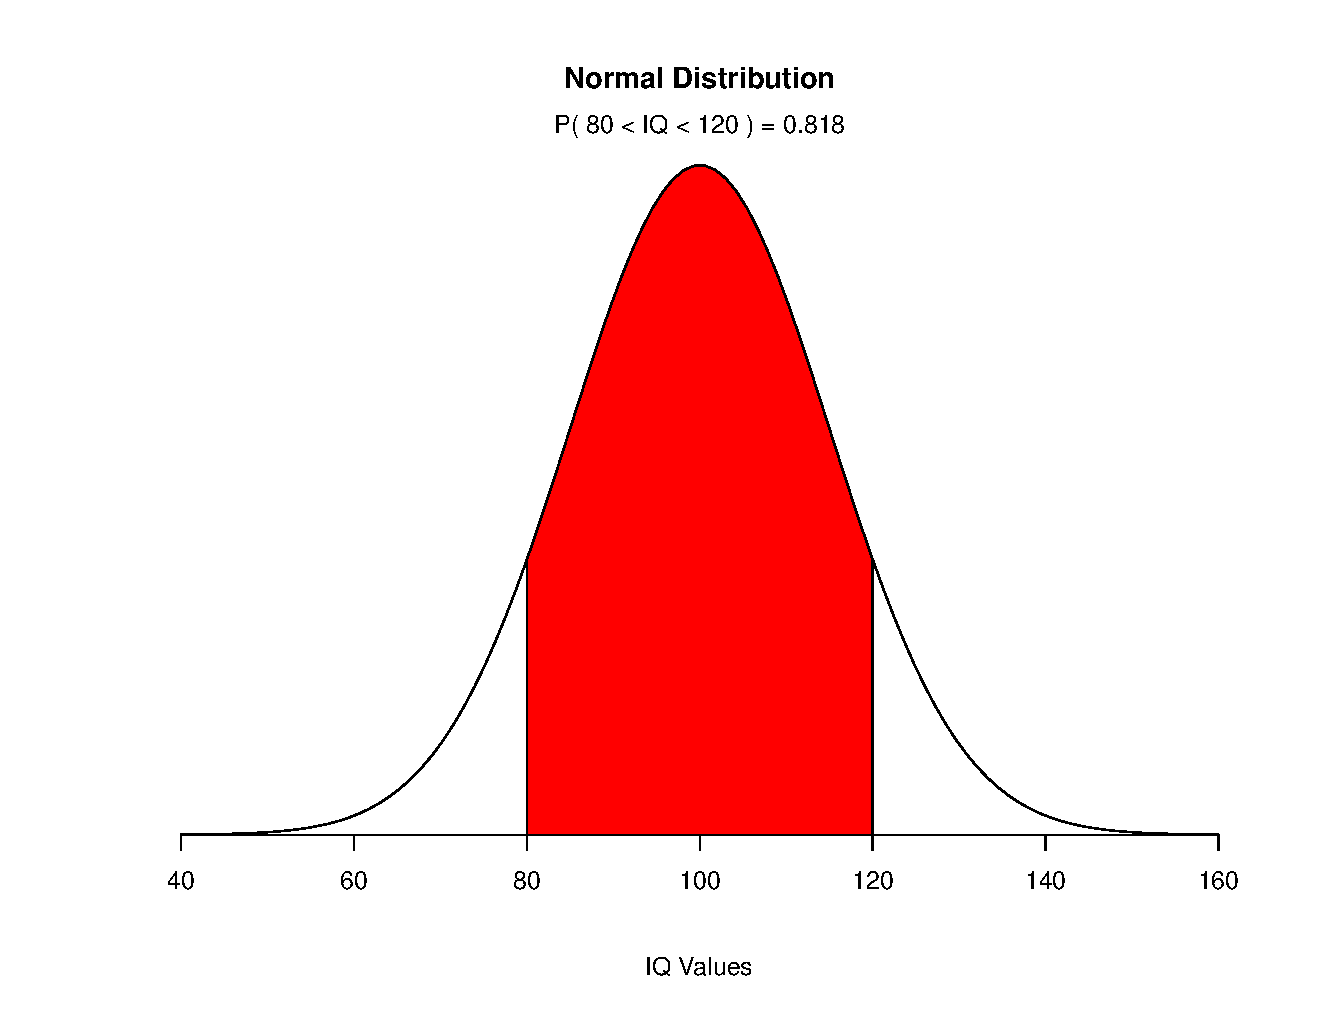
\includegraphics[width=0.85\textwidth]{img/cap02/normal}
  \caption[Distribución normal]{Gráfica de una distribución normal. Fue creado usando el siguiente \href{https://www.statmethods.net/advgraphs/probability.html}{script en R}.}
\end{figure}

Por regla general, lo mejor es usar imágenes de tipo vectorial.
Mi tipo de formato preferido es \verb|*.eps| y recomiendo usar \href{https://ipe.otfried.org/}{IPE} o \href{https://inkscape.org/}{InkScape}, pero otros formatos vectoriales populares para imágenes son el \verb|*.pdf| y \verb|*.svg|.

\section{Subfiguras}

También es posible poner figuras, compuestas de varias subfiguras.
Cada subfigura tiene su propio pié y hay un pié de fígura extra para todo el grupo.
Posteriormente, es posible referirse a toda la figura así: Véase la  Figura~\ref{fig:two} ó referirte a una subfigura así:
Vea la Sub Fígura~\ref{fig:2b}.

\begin{figure}[htp]
 \centering
 \begin{subfigure}[b]{0.45\textwidth}
   
\includegraphics[width=\textwidth]{img/cap02/ambiente}
   \caption{Componente de reflexión ambiental.}
 \label{fig:2a}
 \end{subfigure}
~
 \begin{subfigure}[b]{0.45\textwidth}
   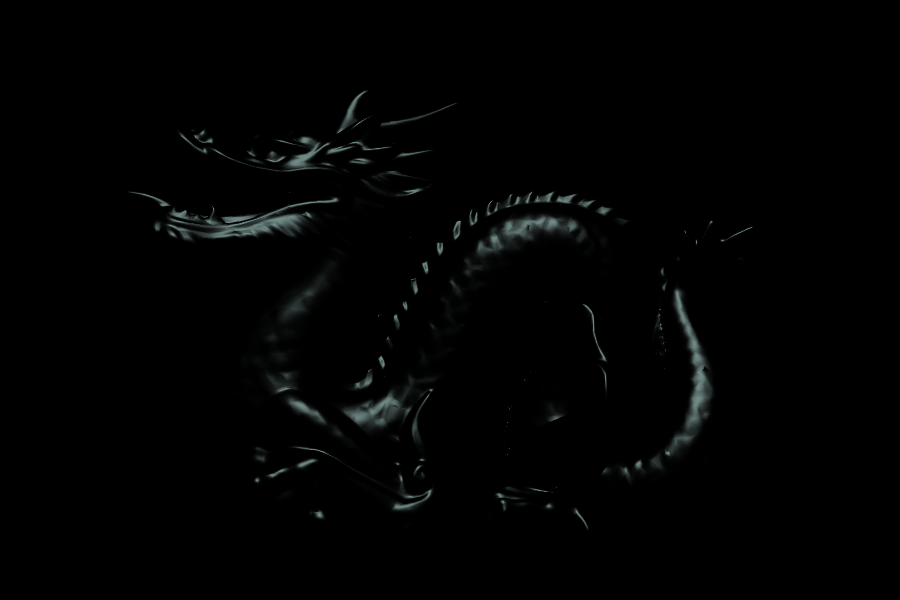
\includegraphics[width=\textwidth]{img/cap02/especular}
   \caption{Componente de reflexión especular.}
   \label{fig:2b}
 \end{subfigure}
\\
 \begin{subfigure}[b]{0.45\textwidth}
   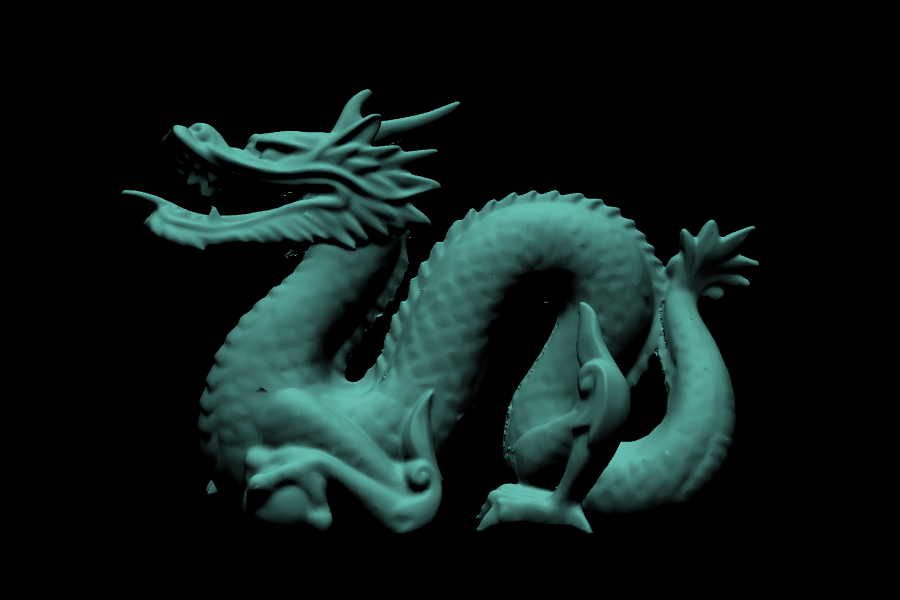
\includegraphics[width=\textwidth]{img/cap02/difuso}
   \caption{Componente de reflexión difuso.}
   \label{fig:2c}
 \end{subfigure}
~
 \begin{subfigure}[b]{0.45\textwidth}
   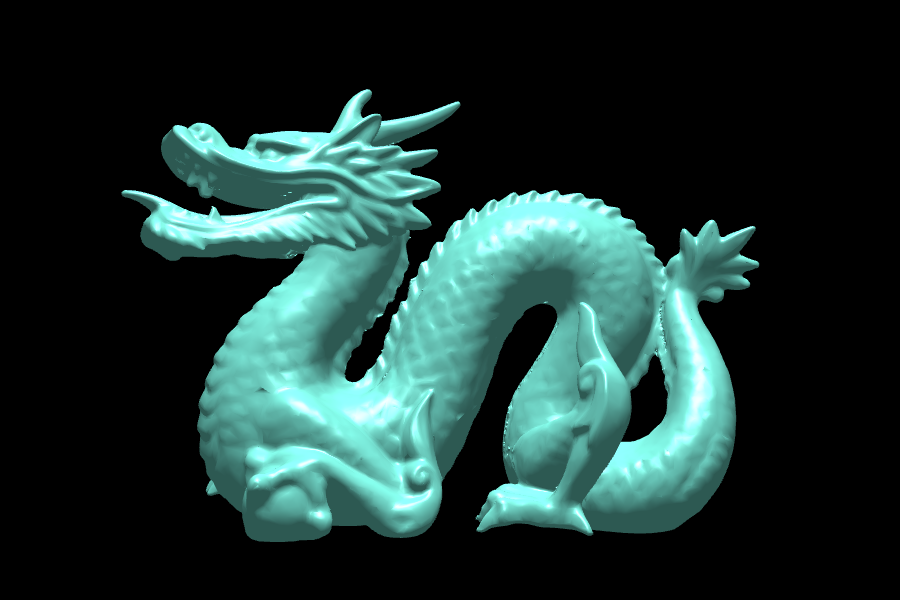
\includegraphics[width=\textwidth]{img/cap02/completo}
   \caption{Modelo completo.}
   \label{fig:2d}
 \end{subfigure}
 \caption[Módelo de iluminación de Phong]{Componentes del módelo de iluminación de Phong.}
 \label{fig:two}
\end{figure}

Por regla general usamos entornos flotantes para poner Figuras, Tablas o pedazos de código.
Esto quiere decir que tenemos que usar especificadores como guías para que \LaTeX{} sepa dónde ponerlos exactamente en el texto.
Puedes consultar más de eso en \href{https://en.wikibooks.org/wiki/LaTeX/Floats,_Figures_and_Captions}{este} wikilibro.

Así es como se cita un libro: éste ejemplo fué tomado de~\cite{Gonzalez:ImagenesDigitales}.
También hay un ejemplo de como hacer que un libro aparezca en las referencias sin que esté citado explícitamente en el texto.

Por último, este es un ejemplo de una tabla muy elegante: Cuadro~\ref{tab:exey}.
Hace uso del paquete \href{https://ctan.org/pkg/booktabs}{booktabs} por que las tablas predeterminadas en \LaTeX se ven muy anticuadas.
Debes de consultar este \href{https://jdhao.github.io/2019/08/27/latex_table_with_booktabs/}{post} y leer esta \href{https://people.inf.ethz.ch/markusp/teaching/guides/guide-tables.pdf}{presentacion} si vas a uasr muchas tablas en tu tesis.

\begin{table}[htb]
  \begin{center}
    \begin{tabular}{l | r r r r r}
      \toprule
      Source & \textbf{DF} & \textbf{SS} & \textbf{MS} & \textbf{F} & \textbf{P-value} \\
      \midrule
      \textbf{Modelo} & 2 & 0.00318564 & 0.00159282 & 7.72 & 0.0014 \\
      \textbf{Error} & 42 & 0.00866760 & 0.00020637 &  & \\
      \midrule
      \textbf{Total} & 44 & 0.01185324 &   &  & \\
      \bottomrule
    \end{tabular}
  \end{center}
\caption{Tabla Anova para un ejercicio imaginario}
\label{tab:exey}
\end{table}


\chapter{Ciencias de la computación}
\label{chap:cs}

\epigraph{\say{We should continually be striving to transform every art into a science: in the process, we advance the art.}}{\textit{Donald Knuth \\ Computer Programming as an Art}}

En éste capítulo, daré algunos tips enfocados a las ciencias de la computación.
Empezamos con el ejemplo de como poner un epígrafe.
Este ejemplo también demuestra como poner \say{comillas} en \LaTeX{}

Primero voy a mostrar cómo incluir algoritmos en forma de pseudocódigo.
Y desde luego se incluyen en el índice y se pueden referencias así: 
El Algoritmo~\ref{alg:euclid} es el primer algoritmo en la historia.
Se puede referenciar una línea del algoritmo.
El ciclo while termina en la línea line~\ref{euclidendwhile}.
Las ídeas las tomé de este enlace \href{https://en.wikibooks.org/wiki/LaTeX/Algorithms#Typesetting_using_the_algorithmicx_package}{wikibook} y de éste \href{https://tex.stackexchange.com/questions/229355/algorithm-algorithmic-algorithmicx-algorithm2e-algpseudocode-confused}{post}.

El entorno de algoritmo como flotante puede salirse de los márgenes de una pagina si no lo configuras correctamente.
Hay un \href{https://tex.stackexchange.com/questions/350434/adjust-width-of-algorithm-float}{truco} para hacerlo entrar en un cierto ancho.
Sin embargo, recomiendo usar el truco como ultima alternativa.
En estos ejemplos no fue necesario.

\begin{algorithm}[H]
\caption{Algoritmo de Euclides}
\label{alg:euclid}
\begin{algorithmic}[1] % The number tells where the line numbering should start 0 for no number
    \Procedure{Euclid}{$a,b$} \Comment{El g.c.d. de $a$ y $b$}
    \State $r\gets a \bmod b$
    \While{$r\not=0$} \Comment{Si $r = 0$ ya tenemos la respuesta}
        \State $a \gets b$
        \State $b \gets r$
        \State $r \gets a \bmod b$
    \EndWhile\label{euclidendwhile}
    \State \textbf{return} $b$\Comment{$gcd = b$}
    \EndProcedure
\end{algorithmic}
\end{algorithm}


\section{Código fuente}
Aquí se muestra cómo incluir código fuente usando el paquete minted.
Este es un ejemplo en el lenguaje C.
\begin{listing}
\begin{minted}{cpp}
int main() {
  printf("hello, world");
  return 0;
}
\end{minted}
\caption{Un programa de ejemplo en C}\label{lst:hello}
\end{listing}

Este es otro ejemplo de cómo incluir Python dentro de un párrafo: \mintinline{python}{print(x**2)}.
Finalmente, lo más útil es incluir el código fuente desde un archivo externo: Vean  el Listado~\ref{lst:example} como ejemplo.
Me ayude muchisimo de \href{https://tex.stackexchange.com/questions/252263/alignment-of-minted-line-numbers}{aquí} y de la \href{https://www.overleaf.com/learn/latex/Code_Highlighting_with_minted}{ayuda de Overleaf}.
Observa la configuración que hice en el archivo \verb|Thesis.sty| para ver cómo obtuve el resultado del Listado~\ref{lst:example}.

\begin{listing}
\inputminted[
  firstline=54, %If you omit this two fields, the whole file is pulled
  lastline=68
  ]{cpp}{src/GccTest.cpp}
  \caption{Una implementación defectuosa de insertion sort}\label{lst:example}
\end{listing}



\chapter*{Conclusiones}
\addcontentsline{toc}{chapter}{Conclusiones}
\markboth{CONCLUSIONES}{CONCLUSIONES}

Las conclusiones tampoco van numeradas y suelen ser breves.
Si te pasas dos hojas creo que deberías volver a escribirlas o pedir que te den un doctorado.

Después sigue la bibliografía, recuerda que se hace uso de biber en vez de bibtex.
Pero afortunadamente en ambas herramientas, el archivo que contiene las fuentes bibliográficas tiene exactamente el mismo formato.
Busca en el archivo \verb|bibliografía.bib| para ver ejemplos de varios tipos de citas.
Como artículos de un journal, libros, tesis, proceedings de una conferencia y un sitio web.



% If you want to change the bibliography style
%\bibliographystyle{ieee_esp}
\nocite{*}

\printbibliography

\addcontentsline{toc}{chapter}{\bibname}

\end{document}
